\chapter{Methods} \label{chapter:methods}

The chosen methodology for this study is Design Science which emphasises the need to design and investigate artifacts in their contexts \cite{wieringa2014design}. It consists of a design and an empirical cycle. The purpose of the former is to improve a problem context with a new or redesigned artifact, while in the latter, the problem is investigated, and its potential treatment is validated concurrently. This strategy seems fitting for our problem in consequence of its practical nature.

The design cycle shares similarities with Action Research \cite{davison2004principles} in which researchers attempt to solve a real-world problem while simultaneously studying the experience of solving said problem. As for the empirical cycle, the pragmatist approach is taken since the value of this research lies in its utility. Moreover, pragmatism adopts an engineering approach to research \cite{shull2007guide}, which happens to be in line with the philosophy of design science. Additionally, as no research method is without flaws, it is imperative to try to compensate for their weaknesses by applying multiple methods. Hence, the study also relies on interviews with professionals to validate the design decisions and determine the generalisability of \textit{GreatAI}.

\section{Design cycle}

The aim of \textit{GreatAI} can be summarised using the terminology of design science in the following way: 
\textit{Facilitate the adoption of AI deployment best practices
by finding a less complex framework design 
which is easier to adopt
in order to decrease the negative externality of misused AI.}

The problem context is the difficulty of responsibly transitioning (while following best practices) from prototype industrial AI applications to production-ready deployments. With the possible treatment being libraries with high-level APIs and a set of default settings. It is important to note that \textit{GreatAI} is merely a proof-of-concept, and its aim is to serve as a proxy for the design decisions behind it. Through this, the design can be indirectly evaluated. Hopefully, a by-product will be a library that can be effectively applied to this problem context.

The practical cases used for the evaluation are further elaborated in Chapter \ref{chapter:case}. In short, they focus on individual components of a growing commercial platform which aims to find tech-transfer opportunities in academic publications. The primary input of the system as a whole is a set PDF files, while the output is a list of metrics describing various aspects of each paper, such as interesting sentences, scientific domains, and contributions. The result also includes a predicted score used for ranking. This ranking is subsequently processed by the business developers of Technology Transfer Offices (TTOs) of multiple Dutch and German universities, who later give feedback on the results.

Overall, this problem context carries the properties of typical industry use cases: it utilises a wide range of natural language processing methods, contains complex interactions between the services, benefits from the integration of end-to-end feedback, and has to provide the clients with a platform that they can rely on within their organisation's core processes. Since the final ranking affects real people, explainability and robustness are also central questions.

\begin{figure}
    \centering
    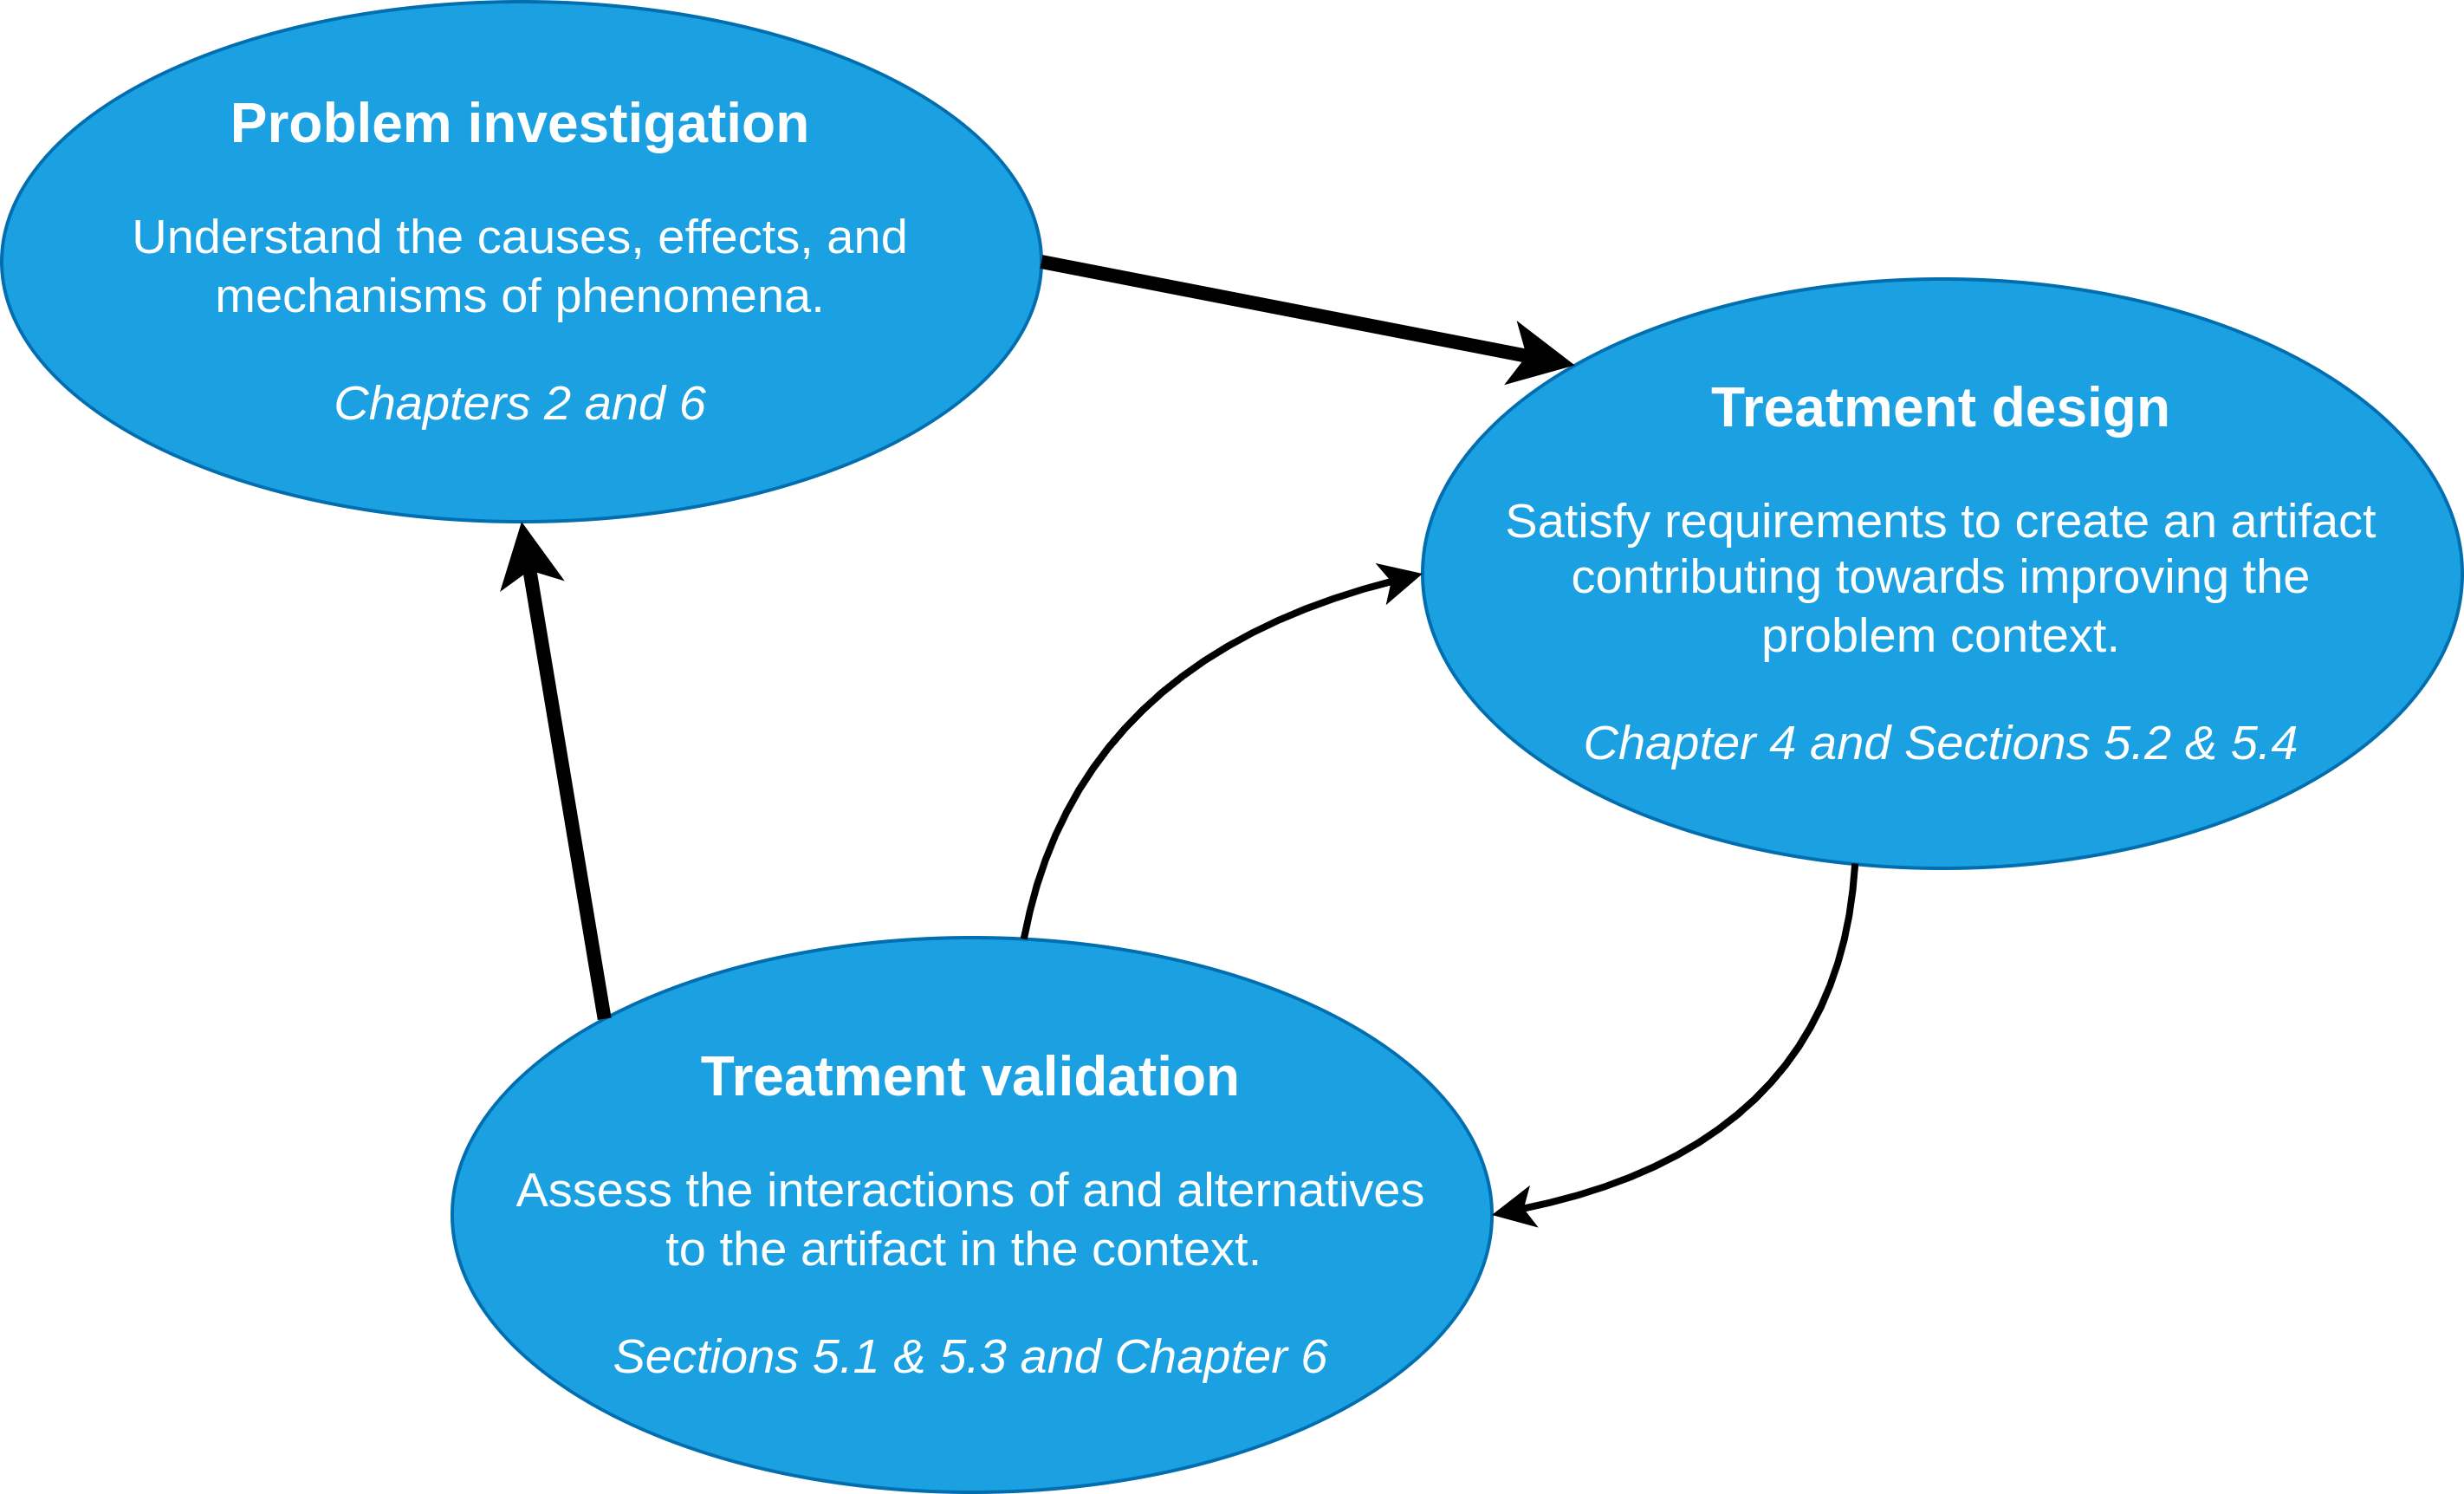
\includegraphics[width=.9\linewidth]{figures/design-cycle.drawio.png}
    \captionsetup{width=.9\linewidth}
    \caption{Implementation of the design cycle of design science \cite{wieringa2014design} for our problem context of AI/ML deployments. The thinner arrows denote smaller but more frequent iterations.}
    \label{fig:design-cycle}
\end{figure}

The goal is to find a simpler, less cognitively-straining-to-use design that still leads to high-quality deployments, the definition of which will be described in Section \ref{section:requirements}. Before generalising, the framework's design is iteratively refined using the feedback acquired from applying it in practical contexts, which in this case are the research and development of a smaller and a more complex AI component using the work-in-progress framework. 

The design cycle summarising the research approach is shown in Figure \ref{fig:design-cycle} indicating the role of the case studies. The concerns arisen in the \textit{Treatment validation} iterations and their short discussions are highlighted in the form of \textit{Design notes}. Afterwards, they are addressed in the following \textit{Treatment design} iteration. This way, the issues are immediately considered and the proposed solutions can be traced back to the problems prompting their introduction.

\section{Applicability \& generalisability} \label{section:interview-setup}

To conclusively answer \textbf{RQ3} and \textbf{RQ4}, we conduct interviews with software engineers and data scientists with varying levels of professional background. The interview candidates were recruited from the recommendations of my acquaintances, who were kindly asked to seek out people from their professional networks with any connection to AI/ML. After the first few interviews, participants were also asked to suggest other candidates, preferably from different subfields. After two iterations of reaching out to potential interviewees personally, ten engineers and researchers eventually responded positively and participated in the study. Albeit the sample size is small, it still represents a wide range of organisation types: experts were included from startups, consultancies, government organisations, and research companies.

First, before their interview, participants are requested to complete a questionnaire (shown in Appendix \ref{appendix:practices}) about their last completed AI project; the questions refer to the best practices implemented by \textit{GreatAI}. They are also advised to take a quick look at the tutorial page of the documentation. 

The interviews are divided into two halves. In the first part, after a brief introduction, interviewees are asked to solve a real-world deployment task by finishing a partially completed example project\footnote{Available at \href{https://github.com/schmelczer/great-ai-interview-task}{github.com/schmelczer/great-ai-interview-task}. The training part of the task has already been done, and the participants only have to deploy the trained classifier.} using \textit{GreatAI}. This is a more straightforward instance of the AI development lifecycle presented in the \textit{GreatAI} tutorials. They are also encouraged to think aloud so their feedback can be noted. Successfully completing the task creates a system implementing a known number of best practices. This way, the added value --- in terms of a larger number of implemented best practices --- can be quantitatively analysed by comparing the qualities of the finished implementation with the previously given answers. The target duration for the interviews is approximately one and a half hours.
 
We follow the guidelines proposed by Halcomb et al. \cite{halcomb2006verbatim} for collecting information from interviews and reporting it. This reflexive, iterative process starts by recording participants (with their permission) and concurrent note-taking. Reflective journaling is immediately done post-interview, which is subsequently extended and revised by listening to the recordings. Afterwards, we interpret the gathered information by applying the methodology of thematic analysis \cite{alhojailan2012thematic}. Thematic analysis is an iterative qualitative investigation technique consisting of labelling, correlating, and structuring the central recurring topics raised during discussions. It has been successfully used in previous software engineering studies for extracting emergent patterns \cite{haakman2021ai,cruz2019catalog}. 

The second half of the one-on-one sessions consists of a short survey allowing us to create the Technology Acceptance Model (TAM) \cite{davis1989perceived} of the problem context. The ultimate goal of the presented library is to help increase the adoption rate of best practices. In order to reach that goal, first, the library itself has to gain adoption. TAM and its numerous variations provide means of measuring users' willingness of adopting new technologies. TAM has been widely applied in literature \cite{marangunic2015technology}, and due to its general psychological origins, it proves to be effective in other areas of technology, not just software \cite{riemenschneider2002explaining}. 

We employ the parsimonious version of TAM, which has been measured to have similar predictive power to that of the original TAM while having fewer variables \cite{wu2011user}. Parsimonious TAM observes three interconnected human aspects that influence the actual behaviour (adoption): \textit{perceived usefulness}, \textit{perceived ease of use}, and \textit{intention to use}. Participants are asked ten questions corresponding to these aspects of their experience using \textit{GreatAI}. The questionnaire is shown in Appendix \ref{appendix:questions}. The internal consistency of the answers is calculated using Cronbach's Alpha \cite{bland1997statistics}, after which we reflect on the responses.
